\documentclass[10pt, oneside]{article} 

\usepackage{algorithm, algorithmicx, algpseudocode, amsmath, amsthm, amssymb,amsfonts,appendix}
\usepackage{bbm, bm,booktabs}
\usepackage{calrsfs,color,cite,caption}
%\usepackage{ctex}
\usepackage{esint,enumitem}
\usepackage{fancyhdr,fontspec,float}
\usepackage{graphicx,graphics,geometry}
\usepackage{hyperref}
\hypersetup{
    hypertex=true,
    colorlinks=true,
    linkcolor=blue,
    filecolor=blue,      
    urlcolor=blue,
    citecolor=blue,
}
\usepackage{indentfirst}
\usepackage{listings}
\definecolor{dkgreen}{rgb}{0,0.6,0}
\definecolor{gray}{rgb}{0.5,0.5,0.5}
\definecolor{mauve}{rgb}{0.58,0,0.82}

\lstset{frame=tb,
	language=Python,
	aboveskip=3mm,
	belowskip=3mm,
	showstringspaces=false,
	columns=flexible,
	basicstyle={\small\ttfamily},
	numbers=none,
	numberstyle=\tiny\color{gray},
	keywordstyle=\color{blue},
	commentstyle=\color{dkgreen},
	stringstyle=\color{mauve},
	breaklines=true,
	breakatwhitespace=true,
	tabsize=3
}
\usepackage[labelfont=bf]{caption}
\usepackage{mathptmx,multirow}
\usepackage{stmaryrd,siunitx,subfigure,setspace}
\usepackage[stable]{footmisc}
\usepackage{tikz,textcomp}
\usetikzlibrary{fit,positioning,arrows,automata}
\usepackage{verbatim}
\usepackage{wasysym}
\usepackage{wrapfig}



\geometry{tmargin=.75in, bmargin=.75in, lmargin=.75in, rmargin = .75in}  


\newtheorem{thm}{$\mathbf{Theorem}$}[section]
\newtheorem{defn}[thm]{$\mathbf{Definition}$}
\newtheorem{conv}[thm]{$\mathbf{Convention}$}
\newtheorem{rem}[thm]{$\mathbf{Remark}$}
\newtheorem{lem}[thm]{$\mathbf{Lemma}$}
\newtheorem{cor}[thm]{$\mathbf{Corollary}$}
\newtheorem{asp}[thm]{$\mathbf{Assumption}$}
\newtheorem*{Proof}{$Proof$}
\renewcommand{\abstractname}{\Large Abstract\\}


\title{
Draft
}
\author{}
\date{Summer 2020}

\begin{document}

\maketitle
\vspace{.25in}
\begin{abstract}
The abstract goes here.
\end{abstract}
\vspace{.25in}

\section{Introduction}
Unconstraint composite optimization has been one of the most essential problems in non-smooth optimization. It is generally stated as follows:

\begin{equation}
\underset{x}{\operatorname{minimize}} \; f(x) \triangleq \phi(x)+h(F(x)),  \; x \in \mathbb{R}^n. 
\label{problem}
\end{equation}

where $\phi: \mathbb{R}^n\rightarrow \mathbb{R}$ is smooth and sometimes 0 in convention. $F: \mathbb{R}^{n} \rightarrow \mathbb{R}^{p}$ is differentiable,$h: \mathbb{R}^{p} \rightarrow \mathbb{R}$ is continuous but non-smooth and in most cases assumed to be nonconvex. Such problem often come with optimization of structured loss function, where $h\circ F$ performs as penalty in order to endow parameters desired structure. For instance, $L^2$ penalty, known as Tikhonov regularization,  provides ridge regression and weight decay in neural network that decrease the scale of parameters. Lasso \cite{Lasso} providing sparsity comes from $L^1$ regularization and ElasticNet \cite{ElasticNet} comes from combination of two. There is also $L^0$ regularization which diminishes rank. When regularization is non-smooth, such as $L^1$ or $L^{\infty}$ norm\cite{NonlinearEqLInfty}, the machine learning problems are exactly composite optimization. 
\par
Plenty of applications in control and signal processing involves composite optimization\cite{CharalambousC}, such as distributed control system\cite{distributedcontrol} and low complexity model\cite{lowcomplexity}. Duchi and Feng \cite{phaseretrieval} considered application in phase retrieval. For true signal $x^*\in \mathbb{R}^n$ and measurement vector $(a_1,\cdots,a_n)$, observation will be $b_i=\phi(<a_i,x^*>)+\epsilon_i,\;i=1,\cdots,n$ where $\phi$ is nonlinear. Ideally the retrieval of $x^*$ is $min_x \frac{1}{n} \sum_{i=1}^{n}\left(\phi\left(\left\langle a_{i}, x\right\rangle\right)-b_{i}\right)^{2}$, which is unfortunately unpractical since observation is usually $b_{i}=\left\langle a_{i}, x^{\star}\right\rangle^{2}$. This leads to optimizing $\frac{1}{n} \sum_{i=1}^{n}\left|\left\langle a_{i}, x\right\rangle^{2}-b_{i}\right|$, again a composite optimization. 
\par

Classical optimization also yield necessity of composite optimization. 
Consider a set of equations $F_i(x)=0,\;i=1,\cdots,n$. Solving this equation is equivalent to optimizing $||F(x)||=||(F_1,\cdots,F_n)||$, as $||\cdot||$ is any norm operator\cite{NonlinearEqLp}. This is a typical composite optimization when the operator is non-smooth. Similarly, consider set of nonlinear inequality constraints $F_i(x)\leq 0,\;i=1,\cdots,n$. A feasible initial point can be obtained by solving $min\;\Sigma ||F^+_i(x)||$, where $F^+_i(x)=max(F_i(x),0)$. 
\par



Theory of composite optimization was first established by A. D. Ioffe \cite{IoffeAD1979}, which has also given conditions for local minimum for sublinear $h$. J. V. Burke\cite{BerkeJV1987} relaxed restriction for $h$ to convex. When F is Lipschitz and Gâteaux differentiable, Jeyakumar and X. Q.  \cite{Lagrange} provided first order Lagrange necessary condition and second order sufficient condition. For cases where $\partial F$ is available, abundant analyses were provided\cite{comp21,comp22,comp56}. \par



In context of numerical algorithm, proximal gradient descent \cite{proximal,accproximal} makes a great substitution after gradient descent fails, though it needs separability of non-smooth term with respect to each variable. By splitting component of smooth and non-smooth in $f$ and impose equality constraint, problem is converted to constraint optimization  and amounts of methods such as ADMM\cite{ADMM} become available. A consequent advantage is that distributed computation is now possible, as problem is decomposed into smooth subproblems or tractable non-smooth ones. However, there is no theoretical guarantees for ADMM when $\phi$ is non-convex. In opposite, method of multipliers \cite{MM} guarantees convergence in non-convex case as well as rigorous parameter tuning framework. But MM requires joint optimization of augmented Lagrange function with respect to all variables, which significantly limits computation speed. Dhingra and Khong\cite{proximalauglag} employ manifold obtained by minimizing variable with respect to non-smooth term, and project augmented Lagrange onto it. This gives continuously differentiable proximal augmented Lagrangian providing distributed computation, rigorous parameter tuning procedure and theoretical guarantees. Bundle methods \cite{bundle,bundle2,bundle3} are a class of most commonly used algorithms in non-convex optimization, even when $\partial F$ is unavailable (derivative free)\cite{bundlefree1,bundlefree2}. 
\par
However, in most cases, $h$ is required to be some specific norm, such as $L^2$ \cite{comp55} and $L^{\infty}$ \cite{comp44,comp56}. This naturally preclude non-convexity of $h$. Larson, Menickellly and Wild \cite{manifoldl1} developed method of $\mathbf{manifold\;sampling}$, a trust-region framework estimating $f(x)$ utilizing estimation of $F(x)$ on nearby manifold and Clarke direction derivative of $h$. Though adopted $h=||\cdot||_1$ as objective function, theoretical analysis and implementation required nothing about convexity. Meanwhile, the algorithm survive in derivative free case and surpass gradient sampling method \cite{grasam1,grasam2} by nonstochasticness. Khan, Larson and Wild \cite{manifoldpiecewiselinear} extended this work by allowing $h$ to be piecewise affine functions. Larson, Menickelly and Zhou \cite{manifold} recently extend $h$ to be any continuous function as long as it is  Clarke sub-derivative is available, though require $\phi=0$. To best of our knowledge, this is the only work for $\mathbf{any\;continuous} $ $h$ and $F$ with $\mathbf{unavailable \;Jacobian}$. 

For this graduate project, we expect to extend work of Larson, Menickelly and Zhou \cite{manifold} to where $\phi$ is a smooth function. Theoretical results are expected to generalize properly, and a software package, ideally in Matlab/Python, is required. New simulations corresponding to the form should be done and, if possible, a real data application employ simply model (Lasso/ ElesticNet) will be done. 

\section{Preliminaries}

\subsection{Problem Setting}

We tend to solve problem 
$$
\underset{x}{\operatorname{minimize}} \; f(x) \triangleq \phi(x)+h(F(x)),  \; x \in \mathbb{R}^n. 
$$
where $\phi: \mathbb{R}^n\rightarrow \mathbb{R}$ is smooth and second order Lipschitz continuous. $F: \mathbb{R}^{n} \rightarrow \mathbb{R}^{p}$ is differentiable, $h: \mathbb{R}^{p} \rightarrow \mathbb{R}$ is continuous but non-smooth and non-convex. 


\subsection{Notations}

All norms in the project are assumed to be $l^2$ norm without specific notation. The closure of set $S$ is denoted as $\mathbf{cl}(S)$. The interior of set $S$ is denoted as $\mathbf{int}(S)$. The convex hull of set $S$ is denoted as $\mathbf{co}(S)$. The image of set $S$ through $F$ is $\mathbf{Im}(S)=:\{F(x)|x\in S\}$. Balls $B(x,\delta)$ are assumed to be closed. 
The generalized Clarke subdifferential of a locally Lipschitz continuous function $f$ at $x$ is 
$$
\partial_{\mathrm{C}} f(x) \triangleq \operatorname{co}\left(\left\{\lim _{y^{j} \rightarrow x} \nabla f\left(y^{j}\right): y^{j} \in D\right\}\right)
$$
where $D$ is some neighborhood. We generally use k on footnote to represent variables in $k^{th}$ iteration. 

\subsection{Definitions and Assumptions}

\begin{defn}
For some constant $\delta_{max}$ and point $x_0$ in $R^n$, define
$$
\mathcal{L}_{\max } \triangleq \bigcup_{x \in \mathcal{L}\left(x^{0}\right)} B \left(x ; \Delta_{\max }\right)
$$
where $\mathcal{L}\left(x^{0}\right)$ is some set we need. This definition will be used as domain of our consideration. 
\end{defn}

\begin{asp}
\label{aspF}
We assume the following about f and F constraint on $\mathcal{L}_{max}$
\begin{itemize}
\item For any $x_0 \in R^n$, set $\mathcal{L}(x_0)=:\{x:f(x)\leq f(x_0)\}$ is bounded
\item $F_i$ is Lipschitz with constant $L_{F_i}$ on $\mathcal{L}_{max}$
\item $\nabla F_i$ is Lipschitz with constant $L_{\nabla F_i}$ on $\mathcal{L}_{max}$
\end{itemize}
\end{asp}

\begin{asp}
We assume the following about smooth function $\phi$.
\begin{itemize}
\item $\phi$ and $\nabla\phi$ can be evaluated inexpensively
\item For any $x_0 \in R^n$, set $\{x:\phi(x)\leq \phi(x_0)\}$ is bounded
\item $\phi$ is Lipschitz with constant $L_{\phi}$ on $\mathcal{L}_{max}$
\item $\nabla \phi$ is Lipschitz with constant $L_{\nabla\phi}$ on $\mathcal{L}_{max}$
\end{itemize}
\end{asp}

\begin{defn}
A function h is a continuous selection on $U \subseteq R^{p}$ if it is continuous on U and 
$$
h(z) \in\left\{h_{j}(z): h_{j} \in \mathfrak{H}\right\}, \quad \forall z \in U
$$
where $\mathfrak{H}$ is a finite set of selection functions. For instance, $h(z)=||z_i||_1$ is a continuous selection provided that it is continuous and $h(z)\in \{\sum\pm z_i\}$
\end{defn}

\begin{defn}
A function h is a continuous selection. Then 
$$
S_{j} \triangleq\left\{z: h(z)=h_{j}(z)\right\}, \quad \tilde{S}_{j} \triangleq \operatorname{cl}\left(\operatorname{int}\left(S_{i}\right)\right), \quad \mathbb{A}(z) \triangleq\left\{j: z \in \tilde{S}_{j}\right\}
$$
$\mathbb{A}(z)$ is active indices set at z. We refer any $h_j$ for which $j\in \mathbb{A}(z)$ as active selection function for h at z. For any set $Z$, let $\mathbb{A}(\mathbb{Z})=\bigcup_{z \in \mathbb{Z}} \mathbb{A}(z)$
\end{defn}

\begin{asp}
We assume the following about h.
\begin{itemize}
\item $\mathbb{A}(z)$ is computable for any z. 
\item $h_i$ is Lipschitz with constant $L_{h_i}$ on $\mathcal{L}_{max}$
\item $\nabla h_i$ is Lipschitz with constant $h_{\nabla F_i}$ on $\mathcal{L}_{max}$
\end{itemize}
\end{asp}

\begin{defn}
A function $m^{F_i}$ is a fully linear model of $F_i$ on $B(x,\Delta)$ if there exists constants $\kappa_{i,ef}$ and $\kappa_{i,eg}$ such that
$$
\begin{aligned}
\left|F_{i}(x+s)-m^{F_{i}}(x+s)\right| \leq \kappa_{i, \mathrm{ef}} \Delta^{2} &,\;\; \forall s \in B(0 ; \Delta) \\
\left\|\nabla F_{i}(x+s)-\nabla m^{F_{i}}(x+s)\right\| \leq \kappa_{i, \mathrm{eg}} \Delta &,\;\; \forall s \in B (0 ; \Delta)
\end{aligned}
$$
\end{defn}

\begin{asp}
\label{secondlip}
For $F=(F_1,\cdots,F_p)$ and its fully linear model $m^F=(m^{F_1},\cdots, m^{F_p})$, $m^F$ is twice continuously differentiable and Lipschitz continuous bounded by constant $\left\|\nabla^{2} m^{F_{i}}(x)\right\| \leq \kappa_{i, \mathrm{mH}}$.
\end{asp}


\begin{defn}
\label{constants}
Here we define some constants to be used, mostly Lipschitz constants.

$$
\begin{array}{c}
L_{F} \triangleq \sqrt{\sum_{i=1}^{p} L_{F_{i}}^{2}} \quad L_{\nabla F} \triangleq \sqrt{\sum_{i=1}^{p} L_{\nabla F_{i}}^{2}}, \quad L_{h} \triangleq \max _{j \in\{1, \ldots,|\mathfrak{H}|\}}\left\{L_{h_{j}}\right\}, \\
\kappa_{\mathrm{f}} \triangleq \sum_{i=1}^{p} \kappa_{i, \mathrm{ef}}, \quad \kappa_{\mathrm{g}} \triangleq \sum_{i=1}^{p} \kappa_{i, \mathrm{eg}}, \quad \quad \kappa_{\mathrm{H}} \triangleq \sum_{i=1}^{p} \kappa_{i, \mathrm{mH}} \\
C \triangleq\left(2 L_{h} \kappa_{\mathrm{g}}+2 L_{\nabla h} L_{F}^{2}+L_{h} L_{\nabla F}+L_{\nabla \phi}\right)
\end{array}
$$
\end{defn}

\begin{defn}
\label{ZDG}
Let $\mathbb{Z}^{k}$ be set of samples 
$$
\mathbb{Z}^{k}=\mathbf{co}\left(\left\{F(y):y\in B(x^k,\Delta_k)\right\}\right)
$$
That is, $\mathbb{Z}^{k}$ includes all points of the form $\alpha F\left(x^{k}\right)+(1-\alpha) F(y) \text { for } \alpha \in[0,1]$. Thus, $\mathbb{Z}^k\subset\mathbf{c o}\left(\operatorname{Im}\left(\mathcal{L}_{\max }\right)\right)$. Let $\mathbb{D}^{k}$ be the set of gradients of linearizations of selection functions.
$$
\mathbb{D}^{k}=\left\{\nabla h_{j}(z): z \in \mathbb{Z}^{k}, j \in \mathbb{A}(z)\right\}
$$
Let $\mathbb{G}^{k}$ be the set of modeled gradients (or generator, as in  \cite{manifold}), of sample set $\mathbb{Z}^{k}$. 
$$
\mathbb{G}^{k}=\left\{\nabla M\left(x^{k}\right) \nabla h_{j}(z)+\nabla \phi: z \in \mathbb{Z}^{k}, j \in \mathbb{A}(z)\right\}
$$
Let $G^{k}$ and $D^{k}$ are matrices with columns that are elements of corresponding set. Also, $G^{k}=\nabla M\left(x^{k}\right) D^{k}+\left( \nabla\phi, \cdots, \nabla \phi \right)$.
\end{defn}


\begin{defn}
\label{g}
Define the approximated gradient $g^k$
\begin{equation}
\label{defg}
g^{k} \triangleq \operatorname{proj}\left(0, \operatorname{co}\left(\mathbb{G}^{k}\right)\right) \in \operatorname{co}\left(\mathbb{G}^{k}\right)
\end{equation}
which is the minimum-norm of element of $\mathbb{G}^{k}$
\end{defn}




\begin{asp}
For $L_F$ in \ref{constants}, we have
$$
F\left(x^{k}\right) \subseteq \mathbb{Z}^{k} \subset \mathcal{B}\left(F\left(x^{k}\right) ; L_{F} \Delta_{k}\right)
$$
\end{asp}



\section{Manifold Sampling}

In this section, we describe manifold sampling algorithm we use. Intuitively, manifold sampling is a model-based derivative free optimization algorithm. Modeling of function $F$ is done by $m^F$ and active selection function $h_j$ is utilized to model $h$. Thus, 
$$
\nabla f=\nabla \phi +\nabla h(F(x))=\nabla \phi +\nabla F(x) \nabla h_{j}(F(x)) \approx \nabla \phi +\nabla m^F(x) \nabla h_{j}(F(x))
$$
Thus by heuristics of gradient descent or trust region method, local minimum can be found. In \ref{ZDG}, $\mathbb{Z}^{k}$ corresponds to derivative free model building part. $\mathbb{D}^{k}$ corresponds to possible $\nabla h$. $\mathbb{G}^{k}$ corresponds to possible $\nabla f$ and $g^k$ in \ref{g} is final approximation of gradient. We now present some subproblem encountered in the algorithm. 


\subsection{Major Components}

\subsubsection{Derivative Free Model}

To acquire model of $F$, we use model-based derivative free techniques. \cite{dfols} utilize fully linearity and least square loss for model building. It worth noting that \cite{dfols} requires only n+1 points to build model for n dimension input. 

\subsubsection{Master Model}

To acquire projection $g^{k} \triangleq \operatorname{proj}\left(0, \operatorname{co}\left(\mathbb{G}^{k}\right)\right) \in \operatorname{co}\left(\mathbb{G}^{k}\right)$, we use convex quadratic optimization 
\begin{equation}
\label{quadratic}
\begin{array}{ll}
\underset{\lambda}{\operatorname{minimize}} & \lambda^{\top}\left(G^{k}\right)^{\top} G^{k} \lambda \\
\text { subject to } & e^{\top} \lambda=1, \lambda \geq 0
\end{array}
\end{equation}
Solving \ref{quadratic} and we can set 
\begin{equation}
\label{gandd}
g^{k} \triangleq G^{k} \lambda^{*} +\nabla\phi \quad \text { and } \quad d^{k} \triangleq D^{k} \lambda^{*}
\end{equation}
Also, we can employ $d^k$ as weights of smooth component $m^{F_i}$
$$
m_{k}^{f}(x) \triangleq \sum_{i=1}^{p}\left[d^{k}\right]_{i} m^{F_{i}}(x)+\phi(x)
$$
A simple observation will be 
$$
\nabla m_{k}^{f}\left(x^{k}\right)=\sum_{i=1}^{p}\left[d^{k}\right]_{i} \nabla m^{F_{i}}\left(x^{k}\right)+\nabla \phi(x^k)=\left(\nabla m^F\left(x^{k}\right) D^{k} +\nabla \phi\right)\lambda^{*}=G^{k} \lambda^{*}=g^{k}
$$

\subsubsection{Sufficient Decrease Condition}

After model building, the master model can be locally optimized by trust-region methods. 
\begin{equation}
\label{minimize}
\underset{s \in B\left(0 ; \Delta_{k}\right)}{\operatorname{minimize}} \quad m_{k}^{f}\left(x^{k}+s\right)
\end{equation}
Exact solution is nor necessary. We provide an available sufficient decrease condition
\begin{equation}
\label{suffdecrease}
\phi(x^k)-\phi(x^k+s^k)+\left\langle m^F\left(x^{k}\right)-m^F\left(x^{k}+s^{k}\right), d^{k}\right\rangle \geq \frac{\kappa_{\mathrm{d}}}{2}\left\|g^{k}\right\| \min \left\{\Delta_{k}, \frac{\left\|g^{k}\right\|}{L_{h} \kappa_{\mathrm{H}}+L_{\nabla \phi}}\right\}
\end{equation}

Note that the sufficient decrease condition \ref{suffdecrease} differs from traditional conditions employed in classical trust-region methods. Instead of measuring the decrease in $m^f(x)$ and $m^f(x+s)$, the left-hand side measures the decrease in terms of the specific convex combination, defined by $d^k$, of the gradients of selection functions at points near $F(x^k)$

\subsubsection{Manifold Sampling Loop}

In \ref{suffdecrease}, $s^k$ suggested by local model based on $\mathbb{Z}^k$ may be defected if $\mathbb{Z}^k$ itself is poor, namely $\mathbb{A}(\mathbb{Z}^k)$ is much too incompatible to $\mathbb{A}(F(x))$. $\mathbb{Z}^k$ thus must be augmented. 

We add new $z$ to $\mathbb{Z}^k$ until the following is satisfied.
$$
\exists z \in \mathbf{co}\left(F(x^k),F(x^k+s^k)\right)\;and\; index\; j \;s.t. 
$$
\begin{equation}
\label{findz}
j\in \mathbb{A}(z)\; and\;\nabla h_{j}(z)^{\top}\left(F(x^{k})-F(x^{k}+s^{k})\right) -\nabla \phi(x^z)\cdot s^k\leq h(F(x^{k}))+\phi(x^k)-h(F(x^{k}+s^{k}))-\phi(x^k+s^k)
\end{equation}

Where $x^z$ is some x that $||F(x)-z||\leq\frac{L_{\nabla F}}{4}||s^k||^2$. Existence of such x is guaranteed by Lemma \ref{approxco}.This condition typically states that there exists j such that $h_j$ performs worse than $d$. 
We also require that there exists a secondary $z'\in \mathbb{Z}^k$ such that 
\begin{equation}
\label{zprime}
j\in\mathbb{A}(z')\;and\;
\left(s^{k}\right)^{\top} \nabla M\left(x^{k}\right)\left(\nabla h_{j}\left(z^{\prime}\right)-d^{k}\right) \leq 0
\end{equation}

Geometrically, this is saying that projection from $s^k$ to generator produced by $d^k$ is better than that produced by $h_j$. 

\subsubsection{Test}
In common with classical trust-region methods, manifold sampling employs a ratio test as a merit criterion. The $\rho_k$ used in the manifold sampling algorithm is the ratio of actual decrease in F to predicted decrease in $m^F$, as weighted by the convex combination of gradients $d^k$.
\begin{equation}
\label{rho}
\rho_{k} \triangleq \frac{\left\langle F\left(x^{k}\right)-F\left(x^{k}+s^{k}\right), d^{k}\right\rangle+\phi(x^k)-\phi(x^k+s^k)}{\left\langle M\left(x^{k}\right)-M\left(x^{k}+s^{k}\right), d^{k}\right\rangle+\phi(x^k)-\phi(x^k+s^k)}
\end{equation}

\subsection{Algorithm}
For detailed pseudo code, check \ref{ap1}.


\subsection{Some Statement}
Here we comment on the algorithm. For upper bound of $\eta_2$, we assume 
\begin{equation}
\label{etamax}
\eta_{\max } \triangleq \min \left\{\frac{1}{L_{\phi}+L_{h} \kappa_{\mathrm{H}}}, \frac{\eta_{1} \kappa_{\mathrm{d}}}{4 C}\right\}
\end{equation}
This might be violated in practice for efficiency. 
We also define acceptable iterations and successful iteration. If in iteration k, $\Delta_k<\eta_2||g^k||$, it is acceptable. If in iteration k, $ \rho_k>\eta_1$, it is successful. 



\section{Theoretical Guarantees}

In this section we present theoretical guarantees stating that under proper parameter settings and initializations, sequences $(x^k, f(x^k))$ converges to local optimum $(x^*,f(x^*))$. We now briefly introduce each lemma's role. Lemma \ref{approxco} provide useful bound for sample set. Lemma \ref{approxg} assures that the way we build master model has a "order-1 subgradient accuracy". Lemma \ref{canfindz} and \ref{algorithmcanfindz} assures proper augmentation exists and can be found by algorithm provided. Lemma \ref{gets} assures that we can always exit loop with some choice of s. Lemma \ref{acciterdecrease} evaluate decrease in each acceptable iteration. Lemma \ref{deltakbdd} provides sufficient condition for successful iteration. Lemma \ref{deltatozero} \ref{liminfg} \ref{substationary} together give a converging subsequence and Theorem \ref{mainthm} states that it converges to Clark sub-stationary point. Since proof is analogous to \cite{manifold}, we only present parts of proof that should be modified. 

\begin{lem}
\label{approxco}
For $z=\alpha F(x)+(1-\alpha)F(y),\; \alpha \in [0,1]$, a path in $\mathbf{c o}\left(\operatorname{Im}\left(\mathcal{L}_{\max }\right)\right)$, we can find a path $\sigma(\alpha),\; \alpha\in[0,1],\;\alpha(0)=x,\;\alpha(1)=y$ in $\mathcal{L}_{max}$ such that 
$$
||\alpha F(x)+(1-\alpha)F(y)-F(\sigma(\alpha))||\leq \frac{1}{4}L_{\nabla F}||x-y||^2
$$

\end{lem}

\begin{proof}
We take $\sigma(\alpha)=\alpha x+(1-\alpha)y$ as example. 
\begin{equation}
\begin{aligned}
&||\alpha F(x)+(1-\alpha)F(y)-F(\alpha x+(1-\alpha)y)||\\
=&||F(x)+(1-\alpha)\nabla F(x)^T(y-x) +(1-\alpha)^2(y-x)^T\nabla^2F(x)(y-x)-(\alpha F(x)+(1-\alpha)F(y))+o(||y-x||^2)||\\
=&||(1-\alpha)(\nabla F(t(y-x))-\nabla F(x))^T(x-y)+(1-\alpha)^2(y-x)^T\nabla^2F(x)(y-x)+o(||y-x||^2)||\\
=&||((1-\alpha)t-(1-\alpha)^2)(y-x)^T\nabla^2F(x)(y-x)+o(||y-x||^2)||\\
\leq&\frac{1}{4}L_{\nabla F}||x-y||^2
\end{aligned}
\end{equation}

\end{proof}

\begin{lem}
\label{approxg}
If all assumption hold, given $x, y\in \mathcal{L}_{max}$ s.t. $||x-y||\leq \Delta$, then for 
$$
\mathbb{G} \triangleq\left\{\nabla M(x) \nabla h_{i}(F(x))+\nabla \phi: i \in I\right\}
$$
$$
\mathbb{H} \triangleq \operatorname{co}\left(\left\{\nabla F(y) \nabla h_{j}(F(y))+\nabla\phi: j \in I\right\}\right)
$$
we have 
$$
\|g-v(g)\| \leq c_{2} \Delta
$$
where
$$
c_{2} \triangleq L_{h}\left(L_{\nabla F}+\kappa_{\mathrm{g}}\right)+L_{F}^{2} L_{\nabla h_{i}}
$$
\end{lem}

\begin{lem}
\label{canfindz}
All assumptions hold, we can find z and j satisfying \ref{findz}.

\end{lem}
\begin{proof}
We define $$
z(\alpha) \triangleq \alpha F(x)+(1-\alpha) F(x+s)
$$
We show by contradiction. Suppose there exists no such $\alpha$ such that $z(\alpha)$ is qualified. Then 
$$
\begin{aligned}
\phi(x)+h(F(x))-\phi(x+s)-h(F(x+s)) & \geq \int_{0}^{1} \inf _{j \in \mathbb{A}(z(\alpha))}\left\{\nabla h_{j}(z(\alpha))^{\top}(F(x)-F(x+s))\right\} -\nabla\phi(x+(1-\alpha) s)\cdot s d \alpha \\
&>\int_{0}^{1}(\phi(x)+h(F(x))-\phi(x+s)-h(F(x+s))) d \alpha\\
&=\phi(x)+h(F(x))-\phi(x+s)-h(F(x+s)) 
\end{aligned}
$$
and thus a contradiction. 
\end{proof}
\begin{lem}
\label{algorithmcanfindz}
All assumptions hold, Algorithm 2 returns z and j in finite time.
\end{lem}


\begin{lem}
\label{gets}
Let $d^k$ and $g^k=\nabla m^Fd^k +\nabla\phi$ be as in \ref{gandd}. If all assumptions hold and \ref{etamax} is satisfied, then
$$
\hat{s}=-\Delta_k\frac{g^k}{||g^k||} 
$$
satisfies \ref{suffdecrease}.
\end{lem}

\begin{Proof}
It is clear that 
\begin{equation}
\label{dbdd}
||d^k||\leq L_h
\end{equation}

From assumption \ref{secondlip} and definition \ref{constants}, 
\begin{equation}
\label{mbdd}
\begin{aligned}
&\left\|M\left(x^{k}\right)+\nabla M\left(x^{k}\right)^{\top} s-M\left(x^{k}+s\right)\right\| \\
\leq & \sum_{i=1}^{p}\left|m^{F_{i}}\left(x^{k}\right)+\nabla m^{F_{i}}\left(x^{k}\right)^{\top} s-m^{F_{i}}\left(x^{k}+s\right)\right| \\
\leq & \sum_{i=1}^{p} \frac{1}{2} \kappa_{i, \mathrm{mH}}\|s\|^{2}=\frac{1}{2} \kappa_{\mathrm{H}}\|s\|^{2}
\end{aligned}
\end{equation}
Combining \ref{dbdd} and \ref{mbdd}, we have 
$$
\begin{aligned}
&\left(d^{k}\right)^{\top}\left(M\left(x^{k}\right)+\nabla M\left(x^{k}\right)^{\top} \hat{s}-M\left(x^{k}+\hat{s}\right)\right) \\
\geq &-\left\|d^{k}\right\|\left\|M\left(x^{k}\right)+\nabla M\left(x^{k}\right)^{\top} \hat{s}-M\left(x^{k}+\hat{s}\right)\right\| \\
\geq &-\frac{1}{2} L_{h} \kappa_{\mathrm{H}}\|\hat{s}\|^{2}=-\frac{1}{2} L_{h} \kappa_{\mathrm{H}} \Delta_{k}^{2}
\end{aligned}
$$
Using \ref{etamax}, we get 
$$
\begin{aligned}
&\phi(x^k)-\phi(x^k+s^k)+\left\langle M\left(x^{k}\right)-M\left(x^{k}+\hat{s}\right), d^{k}\right\rangle \\
\geq&-\nabla\phi(x^k)\cdot \hat{s}-\frac{1}{2}L_{\nabla \phi}\hat{s}^Ts-\left(d^{k}\right)^{\top} \nabla M\left(x^{k}\right)^{\top} \hat{s}-\frac{1}{2} L_{h} \kappa_{\mathrm{H}} \Delta_{k}^{2} \\
=&-\left(g^{k}\right)^{\top} \hat{s}-\frac{1}{2} L_{h} \kappa_{\mathrm{H}} \Delta_{k}^{2}=\left\|g^{k}\right\| \Delta_{k}-\frac{1}{2} L_{h} \kappa_{\mathrm{H}} \Delta_{k}^{2} -\frac{1}{2}L_{\nabla \phi}\Delta_k^2\\
\geq &\left\|g^{k}\right\| \Delta_{k}-\frac{1}{2}\left\|g^{k}\right\| \Delta_{k}=\frac{1}{2}\left\|g^{k}\right\| \Delta_{k} \\
\geq &\frac{\kappa_{\mathrm{d}}}{2}\left\|g^{k}\right\| \min \left\{\Delta_{k}, \frac{\left\|g^{k}\right\|}{L_{\nabla\phi}+L_{h} \kappa_{\mathrm{H}}}\right\}
\end{aligned}
$$
$\hfill\blacksquare$
\end{Proof}

\begin{lem}
\label{acciterdecrease}
All assumption hold. If iteration k of Algorithm 1 is acceptable, then for C in \ref{constants}
\begin{equation}
\label{iterationdecrease}
\phi(x^k) +h(F(x^{k}))-\phi(x^k+s^k)-h(F(x^{k}+s^{k})) \geq\left(d^{k}\right)^{\top}\left(F(x^{k})-F(x^{k}+s^{k})\right)-\nabla\phi(x^k)\cdot s-C \Delta_{k}^{2}
\end{equation}
\end{lem}

\begin{Proof}
We first show that \ref{zprime} always holds. In \ref{zprime}, if z' is found then it is naturally true. Else, we have  $s^{k}=-\Delta_{k} \frac{g^{k}}{\left\|g^{k}\right\|}$. From classical projection theory and \ref{defg}
$$
\begin{aligned}
&\left(\nabla h_{j}\left(z^{\prime}\right)-d^{k}\right)^{\top} \nabla m^F(x^{k})^{\top} s^{k}\\
=&-\left(\nabla h_{j}\left(z^{\prime}\right)-d^{k}\right)^{\top} \nabla m^F(x^{k})^{\top} \Delta_{k} \frac{g^{k}}{\left\|g^{k}\right\|} \\
=&positiveconst\cdot\left[\left(\nabla\phi(x^k)+d^{k} \nabla m^F(x^{k})^{\top}\right) g^k-\left(\nabla\phi(x^k)+\nabla h_{j}\left(z^{\prime}\right) \nabla m^F(x^{k})^{\top}\right) g^k\right]\\
\leq&0
\end{aligned}
$$

From assumption \ref{aspF} and \ref{constants}, 
$$
\left|F(x^{k}+s^{k})-F(x^{k})-\nabla F(x^{k})^{\top} s^{k}\right| \leq \frac{L_{\nabla F}}{2}\left\|s^{k}\right\|^{2}
$$
Thus
$$
\begin{array}{l}
\left(\nabla h_{j}(z)-d^{k}\right)^{\top}\left(F(x^{k}+s^{k})-F(x^{k})-\nabla F(x^{k})^{\top} s^{k}\right) \\
\leq\left\|\nabla h_{j}(z)-d^{k}\right\|\left\|F(x^{k}+s^{k})-F(x^{k})-\nabla F(x^{k})^{\top} s^{k}\right\| \\
\leq\left(2 L_{h}\right) \frac{L_{\nabla F}}{2}\left\|s^{k}\right\|^{2}
\end{array}
$$
which leads to 
$$
\begin{aligned}
& \phi(x^k+s^k)+h(F(x^{k}+s^{k}))-\phi(x^k)-h(F(x^{k}))-\nabla\phi(x^k)\cdot s-\left(d^{k}\right)^{\top}\left(F(x^{k}+s^{k})-F(x^{k})\right) \\
\leq &\left(\nabla h_{j}(z)-d^{k}\right)^{\top}\left(F(x^{k}+s^{k})-F(x^{k})\right) +\phi(x^k+s^k)-\phi(x^k)-\nabla\phi(x^z)\cdot s\\
= &\left(\nabla h_{j}(z)-d^{k}\right)^{\top}\left(F(x^{k}+s^{k})-F(x^{k})\right) +s^T\nabla^2\phi (s-x^z+x)\\
\leq &\left(\nabla h_{j}(z)-d^{k}\right)^{\top} \nabla F(x^{k})^{\top} s^{k}+\left(L_{h} L_{\nabla F}+L_{\nabla \phi}\right)\left\|s^{k}\right\|^{2} \\
=&\left(\nabla h_{j}\left(z^{\prime}\right)-d^{k}\right)^{\top} \nabla F(x^{k})^{\top} s^{k}+\left(\nabla h_{j}(z)-\nabla h_{j}\left(z^{\prime}\right)\right)^{\top} \nabla F(x^{k})^{\top} s^{k}+\left(L_{h} L_{\nabla F}+L_{\nabla \phi}\right)\left\|s^{k}\right\|^{2} \\
\leq &\left(\nabla h_{j}\left(z^{\prime}\right)-d^{k}\right)^{\top}\left(\nabla m^F(x^{k})^{\top} s^{k}+\left(\nabla F(x^{k})-\nabla m^F(x^{k})\right)^{\top} s^{k}\right) \\
&+2 L_{\nabla h} L_{F}^{2} \Delta_{k}^{2}+L_{\nabla\phi}\Delta_k^2+L_{h} L_{\nabla F} \Delta_{k}^{2} \\
=&\left(\nabla h_{j}\left(z^{\prime}\right)-d^{k}\right)^{\top} \nabla m^F(x^{k})^{\top} s^{k}+\left(\nabla h_{j}\left(z^{\prime}\right)-d^{k}\right)^{\top}\left(\nabla F(x^{k})-\nabla m^F(x^{k})\right)^{\top} s^{k} \\
&+2 L_{\nabla h} L_{F}^{2} \Delta_{k}^{2}+L_{\nabla\phi}\Delta_k^2+L_{h} L_{\nabla F} \Delta_{k}^{2} \\
\leq & 0+2 L_{h} \kappa_{g} \Delta_{k}^{2}+2 L_{\nabla h} L_{F}^{2} \Delta_{k}^{2}+L_{\nabla\phi}\Delta_k^2+L_{h} L_{\nabla F} \Delta_{k}^{2} \\
=& C \Delta_{k}^{2}
\end{aligned}
$$
$\hfill\blacksquare$
\end{Proof}

\begin{lem}
All assumptions hold. For acceptable iterations, if 
\begin{equation}
\label{deltakbdd}
\Delta_{k}<\frac{\kappa_{\mathrm{d}}\left(1-\eta_{1}\right)}{4 \kappa_{\mathrm{f}} L_{h}}\left\|g^{k}\right\|
\end{equation}
then $\rho_k>\eta_1$ in Algorithm 1, and the iteration is successful. 
\end{lem}


\begin{lem}
\label{deltatozero}
All assumption hold. If $\{x^k,\Delta_k\}$ is generated by Algorithm 1, then the sequence $\{f(x^k)\}$ is nonincreasing and $\lim_k \Delta_k=0$.
\end{lem}
\begin{Proof}
We show here that f is non-increasing. Rest of the proof  is analogous to \cite{manifold}. If an iteration is unsuccessful, then $x^{k+1}=x^k$, therefore $f(x^{k+1})=f(x^k)$. If it is successful, 
$$
\begin{aligned}
f(x^{k})-f(x^{k+1}) & \geq\left(d^{k}\right)^{\top}\left(F(x^{k})-F(x^{k+1})\right)-\nabla\phi(x^z)\cdot s-C \Delta_{k}^{2} \\
&\geq \left(d^{k}\right)^{\top}\left(F(x^{k})-F(x^{k+1})\right)+\phi(x^k)-\phi(x^k+s^k)-L_{\nabla\phi}\Delta_k^2-C \Delta_{k}^{2} \\
&=\rho_{k}\left[\left(d^{k}\right)^{\top}\left(m^F(x^{k})-m^F(x^{k+1})\right)+\phi(x^k)-\phi(x^k+s^k)\right]-L_{\nabla\phi}\Delta_k^2-C \Delta_{k}^{2} \\
& \geq \rho_{k} \frac{\kappa_{\mathrm{d}}}{2}\left\|g^{k}\right\| \min \left\{\Delta_{k}, \frac{\left\|g^{k}\right\|}{L_{h} \kappa_{\mathrm{H}}+L_{\nabla\phi}}\right\}-L_{\nabla\phi}\Delta_k^2-C \Delta_{k}^{2} \\
&=\rho_{k} \frac{\kappa_{\mathrm{d}}}{2}\left\|g^{k}\right\| \Delta_{k}-C \Delta_{k}^{2}>\eta_{1} \frac{\kappa_{\mathrm{d}}}{2}\left\|g^{k}\right\| \Delta_{k}-L_{\nabla\phi}\Delta_k^2-C \Delta_{k}^{2} \\
&>\eta_{1} \frac{\kappa_{\mathrm{d}}}{2} \frac{4 C}{\eta_{1} \kappa_{\mathrm{d}}} \Delta_{k}^{2}-L_{\nabla\phi}\Delta_k^2-C \Delta_{k}^{2}=C \Delta_{k}^{2}-L_{\nabla\phi}\Delta_k^2>0
\end{aligned}
$$
$\hfill\blacksquare$
\end{Proof}

\begin{lem}
\label{liminfg}
For sequence in Lemma \ref{deltatozero}, we have 
$$
\liminf_{k\to \infty} ||g^k||=0
$$
\end{lem}

\begin{lem}
\label{substationary}
For sequence in Lemma \ref{deltatozero}, there is a infinite subsequence of acceptable iterations $\{k_j\}$ such that 
$$
\lim _{j \rightarrow \infty}\left\|g^{k_{j}}\right\|=0
$$
and $\{x^{k_j}\}$ converge to some $x^*$. What is more, $0\in \partial_Cf(x^*)$.
\end{lem}


\begin{thm}
\label{mainthm}
All assumptions hold. For a sequence generated by Algorithm 1, its cluster point is Clark sub-stationary. 
\end{thm}

\section{Simulations}
We present numerical simulation results in the section. We first illustrate with classical examples that manifold sampling is computational efficient and considerably precise. We also adopt benchmark from \cite{benchmark} consisting of ten non-smooth optimization problems. We pay special attention to locally convergence and illustrate performance under far starting point. Then we test performance of MS under non-convex non-smooth situation. At last, we combine MS with neural network parameter optimization. 
\subsection{$L^1$ Norm}
We first consider a simple situation
\begin{equation}
\label{testfunc1}
\phi(x)+h(F(x))=||x||_2+||((x_2-x_1^2)^2+(1-x_1)^2,x_3)||_1,\;x\in \mathbb{R}^3
\end{equation}
where h is $L^1$ norm and $\phi : \mathbb{R}^3 \to \mathbb{R}^2 $ is Rosenbrock test function on its first element. The third element is additive separable and take 0 as optimum. Function value with respect to $x_1$ and $x_2$ is as Figure \ref{fig:function}.

\begin{figure}[h]
\centering
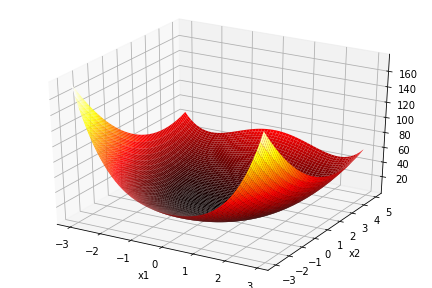
\includegraphics[scale=.6]{function.png}
\caption{Function value w.r.t. $x_1$ and $x_2$.}
\label{fig:function}
\end{figure} 

Noting that this is generally convex, we don't post result about locally convergence here. For hyperparameters, we set $\eta_1=0.1,\;\eta_2=1,\;\kappa_d=10^{-4},\;\kappa_H=1,\;\gamma_d=0.5,\;\gamma_i=1.5,\;\Delta_{max}=10^4,\;\Delta_{min}=10^{-13}$. Initial $x_0$ is chosen random from standard Gaussian. If algorithm performs at most 3000 iteration. From a perspective of practice, we also set termination condition that algorithm shuts if $\left|f(x^k)-f(x^{k+1})\right|<conv\_tol=10^{-9}$ for several successive k (three for us). We especially care for number of points that is used to build local derivative free model since it greatly effect efficiency and precision. Figure \ref{fig:npt} shows performance of model under different number setting. We set number of points to 10 in following experiments because it achieves both reasonable precision and is comparably fast. 

\begin{figure}[H]
\centering

\subfigure{
  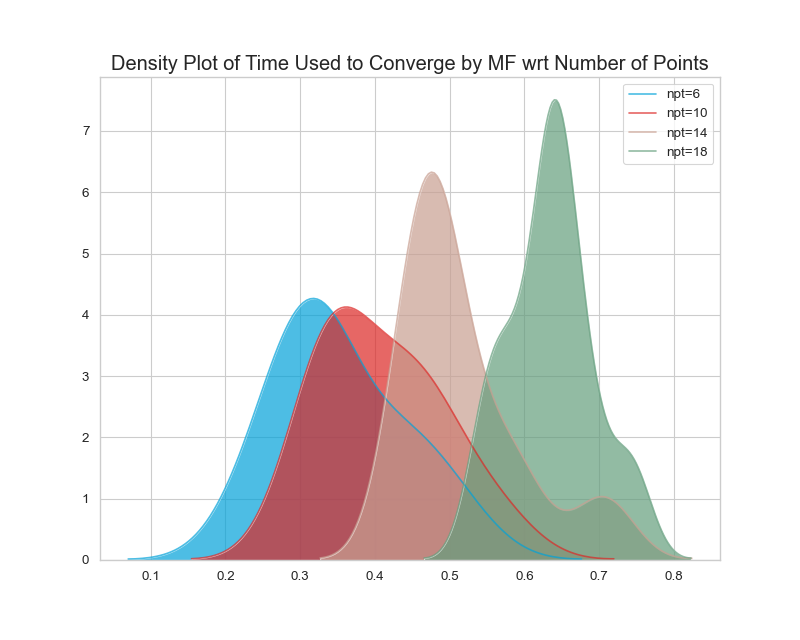
\includegraphics[width=0.4\linewidth]{npttime.png}
  }
  \subfigure{
  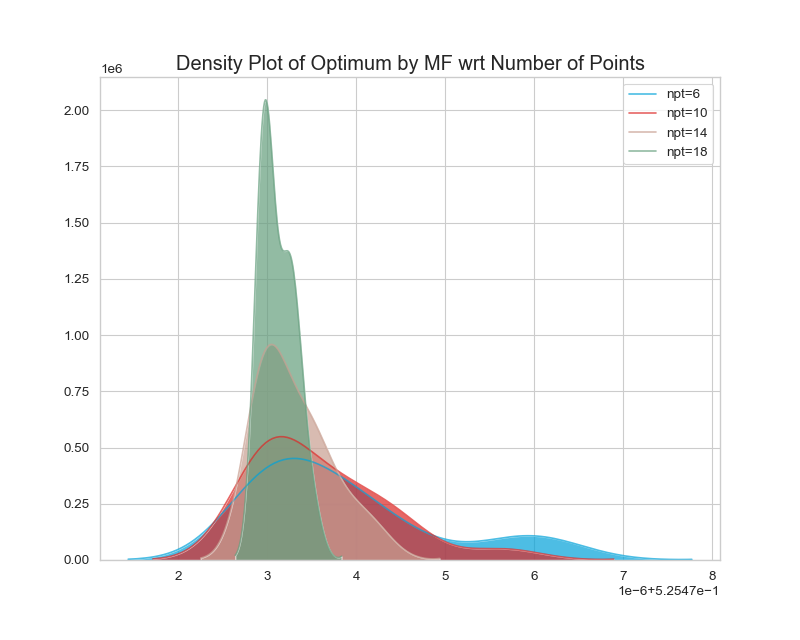
\includegraphics[width=0.4\linewidth]{nptvalue.png}
   }
   \caption{(Best viewed in color) Distribution of time and returned objective function value. Unsurprisingly, increasing number of points leads to more robust model with trade off in time. }
   \label{fig:npt}
  \end{figure}

We adopt two simple benchmarks. One is least square derivative free optimization tool box by \cite{dfols}, to compare manifold sampling and other derivative free methods. Another is simply gradient descent with implementation in PyTorch. Note that this is possible only if function h is piecewise smooth and that F(x) falling in non-smooth region has measure zero. Use of PyTorch is for further work of combining MF and neural network. Figure \ref{fig:compare} presents their performance and shows superiority of MF. 

\begin{figure}[H]
\centering

\subfigure{
  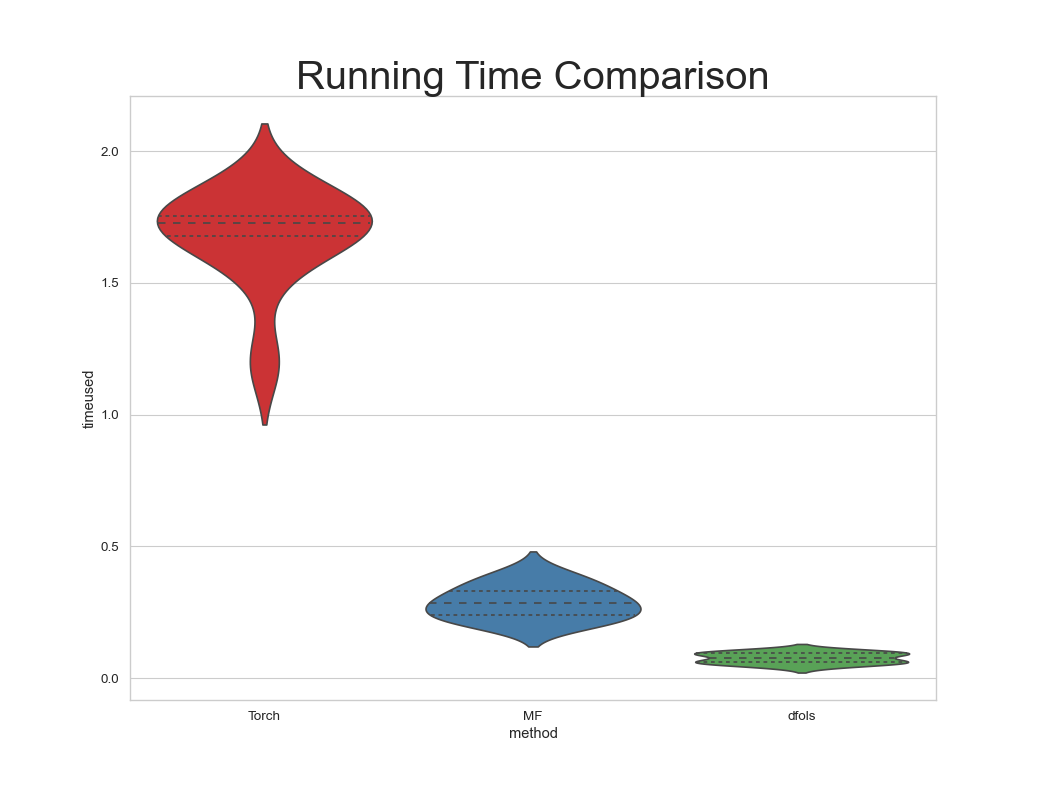
\includegraphics[width=0.4\linewidth]{timecompare.png}
  }
  \subfigure{
  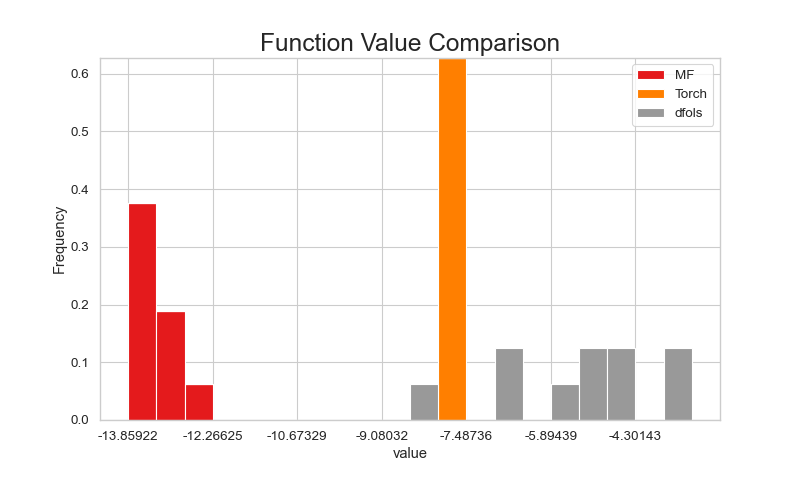
\includegraphics[width=0.5\linewidth]{valuecompare.png}
   }
   \caption{(Best viewed in color) Comparison result of three model. Function value is viewed in log scale of difference with oracle obtained by grid search. MF achieves best precision in relatively short time. }
   \label{fig:compare}
  \end{figure}
  
However, Rosenbrock function in \ref{testfunc1} is non-negative and thus $L^1$ norm posed is meaningless. Thus we change the test problem to 
\begin{equation}
\label{testfunc2}
\phi(x)+h(F(x))=||x||_2+||((x_2-x_1^2)^2-(1-x_1)^2,x_3)||_1,\;x\in \mathbb{R}^3
\end{equation}
This is a non-convex problem and its behavior around the origin is shown in \ref{fig:function2}.

\begin{figure}[H]
\centering

\subfigure{
  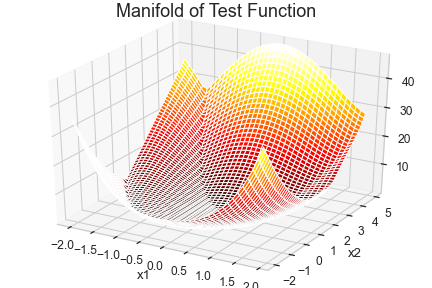
\includegraphics[width=0.4\linewidth]{function2.png}
  }
  \subfigure{
  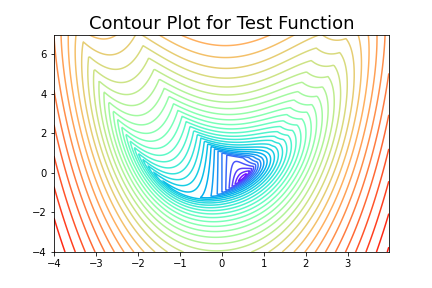
\includegraphics[width=0.4\linewidth]{contour.png}
   }
   \caption{(Best viewed in color) Test function plotting. Left is plot of manifold around origin, right is contour plot of log value of test function. }
\label{fig:function2}
  \end{figure}

For performance on this problem, check \ref{ap2}.


\subsection{Benchmark Problem Set}
We adopt \cite{benchmark} as benchmark. The problem set is especially designed for non-smooth optimization and can provide problem of any dimension scale. For details, please check \ref{ap3}. The result is displayed in Table \ref{tab:result}. We emphasize that most, if not all, of the original problems was formed in low dimension with n=2, in which cases manifold sampling performed pretty well. Yet high dimension experiments were done for further exploration. 

% Please add the following required packages to your document preamble:
% \usepackage{multirow}
\begin{table}[]
\centering
\begin{tabular}{c|c|ccccccc}
\hline
Problem                                                                              & Curvature                 & n   & Convergence & \begin{tabular}[c]{@{}c@{}}Reach \\ Optimum\end{tabular} & Error & Liminf Error & Time(s) & Iteration \\ \hline
\multirow{4}{*}{\begin{tabular}[c]{@{}c@{}}Generalization of \\ MAXQ\end{tabular}}   & \multirow{4}{*}{2}        & 2   & Y           & Y                                                        & -9    & -9           & 1.71    & 150       \\ 
                                                                                     &                           & 5   & Y           & Y                                                        & -9    & -9           & 3.59    & 300       \\ 
                                                                                     &                           & 10  & Y           & Y                                                        & -9    & -9           & 6.57    & 500       \\ 
                                                                                     &                           & 100 & Y           & Y                                                        & -5    & -5           & 140     & 3000      \\ \hline
\multirow{4}{*}{\begin{tabular}[c]{@{}c@{}}Generalization of \\ MXHILB\end{tabular}} & \multirow{4}{*}{1}        & 2   & Y           & Y                                                        & -6    & -6           & 5.46    & 300       \\  
                                                                                     &                           & 5   & Y           & Y                                                        & -5    & -5           & 51      & 3000      \\  
                                                                                     &                           & 10  & Y           & Y                                                        & -5    & -5           & 107     & 3000      \\  
                                                                                     &                           & 100 & Y           & Y                                                        & -3    & -5           & 5598    & 3000      \\ \hline
\multirow{4}{*}{Chained LQ}                                                          & \multirow{4}{*}{2(n-1)}   & 2   & Y           & Y                                                        & -6    & -6           & 2.74    & 100       \\  
                                                                                     &                           & 5   & Y           & Y                                                        & -3    & -5           & 112     & 3000      \\  
                                                                                     &                           & 10  & Y           & \textit{\textbf{N}}                                      &       & -5           & 180     & 3000      \\  
                                                                                     &                           & 100 & N           & Y                                                        &       & -5           &         &           \\ \hline
\multirow{4}{*}{Chained CB3 1}                                                       & \multirow{4}{*}{12(n-1)}  & 2   & Y           & Y                                                        & -8    & -8           & 21.4    & 1000      \\  
                                                                                     &                           & 5   & Y           & \textit{\textbf{N}}                                      & -1    & -4           & 20.0    & 250       \\  
                                                                                     &                           & 10  & N           & N                                                        &       & -1           &         &           \\  
                                                                                     &                           & 100 & N           & N                                                        &       & -1           &         &           \\ \hline
\multirow{4}{*}{\begin{tabular}[c]{@{}c@{}}Chained \\ CB3 2\end{tabular}}            & \multirow{4}{*}{12}       & 2   & Y           & Y                                                        & -9    & -9           & 27.3    & 1450      \\  
                                                                                     &                           & 5   & Y           & Y                                                        & -3    & -4           & 61.6    & 3000      \\  
                                                                                     &                           & 10  & Y           & Y                                                        & -3    & -3           & 80.4    & 3000      \\  
                                                                                     &                           & 100 & Y           & Y                                                        & -3    & -3           & 590     & 3000      \\ \hline
\multirow{4}{*}{\begin{tabular}[c]{@{}c@{}}Number of \\ Active Faces\end{tabular}}   & \multirow{4}{*}{$\infty$} & 2   & Y           & Y                                                        & -9    & -9           & 3.30    & 130       \\  
                                                                                     &                           & 5   & N           & N                                                        &       & -1           &         &           \\  
                                                                                     &                           & 10  & N           & N                                                        &       & -1           &         &           \\  
                                                                                     &                           & 100 & N           & N                                                        &       & -1           &         &           \\ \hline
\multirow{4}{*}{Chained Milfflin}                                                    & \multirow{4}{*}{2(n-1)}   & 2   & Y           & Y                                                        & -9    & -9           & 31.3    & 1600      \\  
                                                                                     &                           & 5   & Y           & Y                                                        & -6    & -6           & 71.7    & 3000      \\  
                                                                                     &                           & 10  & N           & N                                                        &       &              &         &           \\  
                                                                                     &                           & 100 & N           & N                                                        &       &              &         &           \\ \hline
\multirow{4}{*}{Chained Crescent 1}                                                  & \multirow{4}{*}{2}        & 2   & Y           & Y                                                        & -9    & -9           & 3.14    & 150       \\  
                                                                                     &                           & 5   & Y           & Y                                                        & -8    & -8           & 22      & 700       \\  
                                                                                     &                           & 10  & Y           & Y                                                        & -7    & -7           & 30      & 1200      \\  
                                                                                     &                           & 100 & Y           & Y                                                        &       & -3           &   90      &    3000       \\ \hline
\multirow{4}{*}{Chained Crescent 2}                                                  & \multirow{4}{*}{2(n-1)}   & 2   & Y           & Y                                                        & -7    & -7           & 2.11    & 150       \\  
                                                                                     &                           & 5   & N           & N                                                        &       & -4           &         &           \\  
                                                                                     &                           & 10  & N           & N                                                        &       & -1           &         &           \\  
                                                                                     &                           & 100 & N           & N                                                        &       & 1            &         &           \\ \hline
\end{tabular}

\caption{Experiment result on benchmark. We test MS on nine problem (there was ten problems in benchmark set but problem 7 is not compatible with our formulation by adopting inseparable non-smoothness and compositeness) with input dimension n=2, 5, 10 and 100 to see how MS perform on high dimension tasks. Midway dimension m is intrinsic as illustrate in \ref{ap3}. We also list out upper bound of $h(L_{\nabla F_i},\cdots)$ at optimum for further use and we call this "curvature". All results are acquired from single trial but every case is guaranteed not to be outlier by at least five additional trials. By convergence we mean whether $x^k$ and $f(x^k)$ is convergent. By reaching optimum we mean that whether $x^k$ and $f(x^k)$ is approaching the global optimum. For all problems, since function has unique global minimum, we would expect convergence implies reaching optimum. However, violation happened in “Chained CB3 1” and "Chained CB3 2". This is not due to occasional numerical error. We further check that curvature around optimum is relatively large, which we blame this situation on. By error we mean the log scale of difference between optimal value and convergent sequence. Note that for problem "Chained Milfflin", we do not have exact extreme value and thus we use the Cauchy limit of sequence if convergent and omit if not. We also add inferior limits here to illustrate potential convergence.Reason for jumping out of convergence lies in two possibilities. One is numerical explosion and the other is F itself. See below for further discussion. By time and iteration we mean period of time and iterations (less than 3000) spent by algorithm. Positions omitted is where filling this position is meaningless, e.g. time for a non-convergent trial. }
\label{tab:result}
\end{table}




We note that in the experiment, some sequence non-convergent sequence will have a convergent subsequence to optimum. We believe the second reason, which is about F, accounts for most cases. For instance, in trials where error is large (or even not convergent) and liminf is small, "Chained CB3 1" "Number of Active Faces" and "Chained Crescent 2", the "curvature" we presented in the table is respectively $12(n-1),\;\infty$ and $2(n-1)$, which is large and makes the bounding effect of curvature useless. Thus it is reasonable for this to happen. For some other intuition, though the three problems all converges for n=2, "Chained CB3 1" and "Chained Crescent 2" has small curvature for small n, thus they still have small liminf for n=5, while "Number of Active Faces" does not. We add here some discussion of performance sensitivity with respect to n. In test set, solution can still be acquired when n=100 for "MAXQ", "MXHILB", "CB3 2" and "Crescent 1", all of which have curvature of constant scale.

\subsection{Nonconvexity}
We argue that, though non-convex, the test function does not have non-convex h, which is one reason that manifold sampling is powerful. Thus we check for general non-convex non smooth function. 
\begin{equation}
\label{testfunc3}
\phi(x)+h(F(x))=-exp(-||x||^2)+h((x_2-x_1^2)^2,(1-x_1)^2), \;x\in \mathbb{R}^2
\end{equation}
$$
h(z)=\sum_{i=1}^m |1-z_i^2|
$$
We present the problem as before in Figure \ref{fig:function3} and solution in \ref{ap4}

\begin{figure}[H]
\centering

\subfigure{
  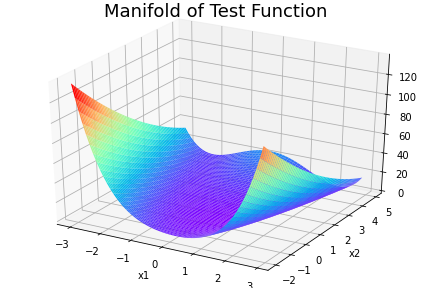
\includegraphics[width=0.4\linewidth]{function3.png}
  }
  \subfigure{
  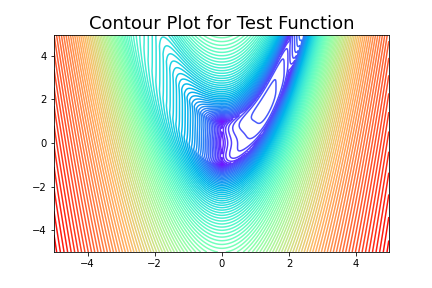
\includegraphics[width=0.4\linewidth]{contourtry.png}
   }
   \caption{(Best viewed in color) Test function plotting. Left is plot of manifold around origin, right is contour plot of log value of test function. The function has five local minimum, (0,0)(0,1)(0,-1)(2,3)(2,5)}
\label{fig:function3}
  \end{figure}
  
  We generate 1000 initial points from uniform distribution $[-3,3]\times [-3,3]$ to test local convergence of MS on non-convex h. In most trials, sequence converges successfully and we present convergence result in Figure \ref{fig:convergence}. Due to limitations in computation resources, we could only use large search step when samples are large. The converging shows territorial property that initial points will converge to closest stationary point. 
  
  \begin{figure}[H]
\centering

  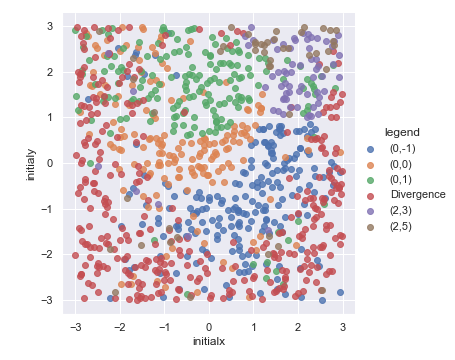
\includegraphics[width=0.8\linewidth]{convergence1.png}

   \caption{(Best viewed in color) We note that in left picture there are many divergent trials still. This is due to searching parameters in \ref{minimize}. Since 1000 experiments are expensive to run, we could only adopt large search steps, which leads to $x^k$s jumping between two "slope" of loss surface. Given enough time and small search step, then would surely converge.}
\label{fig:convergence}
  \end{figure}
  

\section{Empirical Study}

For real data application, we use MS to do regression task using feed forward neural network. The dataset we use is diabetes dataset from \cite{lars}. There are ten baseline variables---age, sex, body-mass index, average blood pressure, and six blood serum measurements serving as independent variables, with the response of interest being a quantitative measure of disease progression one year after baseline. 442 samples are included. We build feed forward neural network with one hidden layer including 10 hidden units using sigmoid function as activation. Since sample size is relatively small, we use gradient descent as a benchmark and examine change of loss through time as in Figure \ref{fig:loss}. In the figure, though unstable, MS is able to beat NN by a lower loss and faster speed. 

  
  \begin{figure}[H]
\centering
  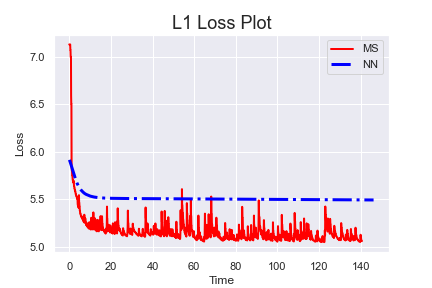
\includegraphics[width=0.8\linewidth]{loss.png}
   \caption{(Best viewed in color). Change of loss in log scale through time. MS rapidly finds minimum better than gradient descent. Note that as naive benchmark, we do not perform batch norm or learning rate tuning, which is unfair for MS since no hyper parameter tuning pipeline has been given. Oscillation of MS is due to that parameter set previously is no longer proper after it falls into region with higher "curvature". }
\label{fig:loss}
\end{figure}


\bibliographystyle{plain}
\bibliography{Proposal.bib}


\newpage
\appendix

 \section{Code}
 \label{ap1}
Pseudo code of main part of manifold sampling is in \ref{algorithm1}. \ref{algorithm2} is grid search method necessary for Algorithm 1. 


\begin{algorithm}
        \caption{Manifold Sampling}
        \label{algorithm1}
        \begin{algorithmic}[1] %每行显示行号
\State  Set $\eta_{1} \in(0,1), \kappa_{\mathrm{d}} \in(0,1), \kappa_{\mathrm{H}} \geq 0, \eta_{2} \in\left(0, \eta_{\max }\right), 0<\gamma_{\mathrm{d}}<1 \leq \gamma_{\mathrm{i}}, \text { and } \Delta_{\max }, \Delta_{\min }>0$
\State Choose $\Delta_0$ in $(0,\Delta_{max}]$ and initialize $x^0$
		  \For{$k= 0 \to K$}
		  \State Build master model $m^F$
		  \State Initialize $\mathbb{Z}^k$ and Form $D^k$
		  \While{true}
		  \State Form $\nabla m^F$
		  \State $G^{k} \gets \nabla M\left(x^{k}\right) D^{k}+(\nabla \phi(x^k),\cdots,\nabla \phi(x^k))$
		  \State Solve \ref{quadratic} for $\lambda^*$
		  \State $d^k\gets D^k \lambda^*$
		  \State $g^k\gets G^k\lambda^*$
		  \If{$\Delta_k<\Delta_{min}$}
		  \State Break
		  \EndIf
		  \If{$\Delta_k<\eta_2||g^k||$}
		  \State Solve \ref{minimize} to get $s^k$
		  \State Get z and j satisfying \ref{findz} using Algorithm 2
		  \If{$j\in \mathbb{A}(\mathbb{Z}^k)$ and no z' satisfies \ref{zprime}}
		  \State $s^k\gets -\Delta_{k} \frac{g^{k}}{\left\|g^{k}\right\|}$
		  \State Get z and j satisfying \ref{findz} using Algorithm 2
		  \EndIf
		  \If{$j\in\mathbb{A}(\mathbb{Z}^k)$}
		  \State Calculate $\rho_k$ using \ref{rho}
		  \State Break
		  \Else
		  \State Update $m^F$ and $Z\mathbb{Z}^k$
		  \State Form $D^k$
		  \EndIf
		  \Else
		  \State $\rho_k\gets 0$
		  \State Break
		  \EndIf
		  \EndWhile
		  \If{$\rho_k>\eta_1>0$}
		  \State $x^{k+1}\gets x^k+s^k$
		  \State $\Delta_{k+1}\gets min\{\gamma_i\Delta_k,\Delta_{max}\}$
		  \Else
		  \State $x^{k+1}\gets x^k$
		  \State $\Delta_{k+1}\gets \gamma_d\Delta_k$
		  \EndIf
		  \EndFor
		  
\end{algorithmic}
\end{algorithm}


\begin{algorithm}	
	
        \caption{Grid Search for z and j}
        \label{algorithm2}
        \begin{algorithmic}[1] %每行显示行号
        \If {$x^z=x$, F(x) and j satisfy \ref{findz}}
        \State\Return{F(x) and j}
        \EndIf
        \If {$x^z=x+s$, F(x+s) and j satisfy \ref{findz}}
        \State\Return{F(x+s) and j}
        \EndIf
        \For{$l=0,\cdots$}
        \State Generate $\{\frac{2 k-1}{2^{l}}: k=1, \ldots, 2^{l-1}\}$
        \For{$k=1, 2, \cdots 2^{l-1}$}
        \State $\alpha\gets\frac{2k-1}{2^l}$
        \State $z(\alpha)\gets\alpha F(x)+(1-\alpha)F(x+s)$
         \If {$x^z=x+(1-\alpha)s,\; z(\alpha)$ and j satisfy \ref{findz}}
        \State\Return{$z(\alpha)$and j}
        \EndIf
        
        \EndFor
        \EndFor
\end{algorithmic}
\end{algorithm}



 \section{Test Performance}
 \label{ap2}
 
 We adopt same procedure for performance test as in Figure \ref{fig:npt2} and \ref{fig:compare2}. 
\begin{figure}[H]
\centering

\subfigure{
  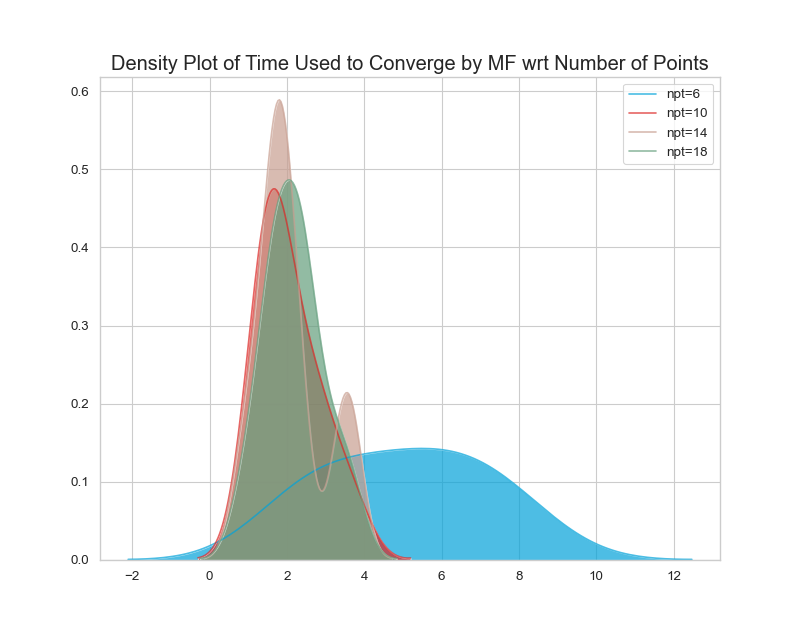
\includegraphics[width=0.4\linewidth]{npttime2.png}
  }
  \subfigure{
  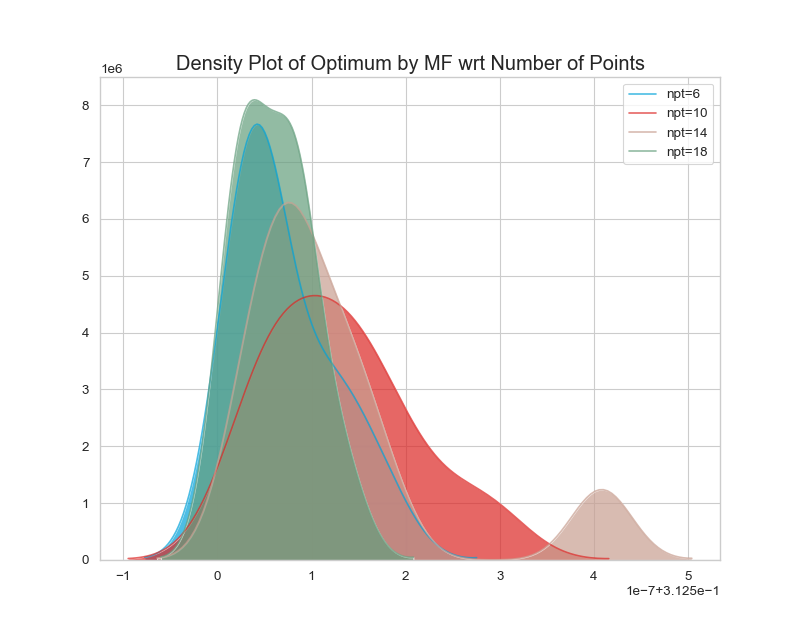
\includegraphics[width=0.4\linewidth]{nptvalue2.png}
   }
   \caption{(Best viewed in color) Distribution of time and returned objective function value. There is one trial for npt=14 that broke down, which led to poor performance. }
   \label{fig:npt2}
  \end{figure}


\begin{figure}[H]
\centering

\subfigure{
  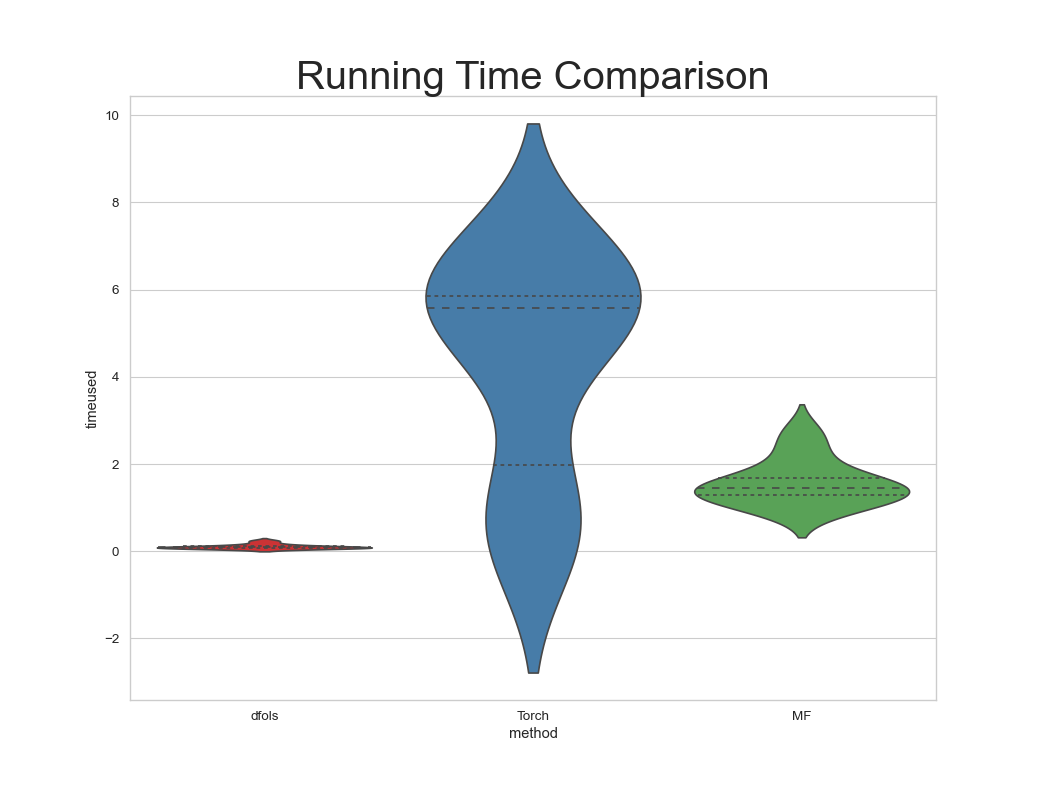
\includegraphics[width=0.4\linewidth]{timecompare2.png}
  }
  \subfigure{
  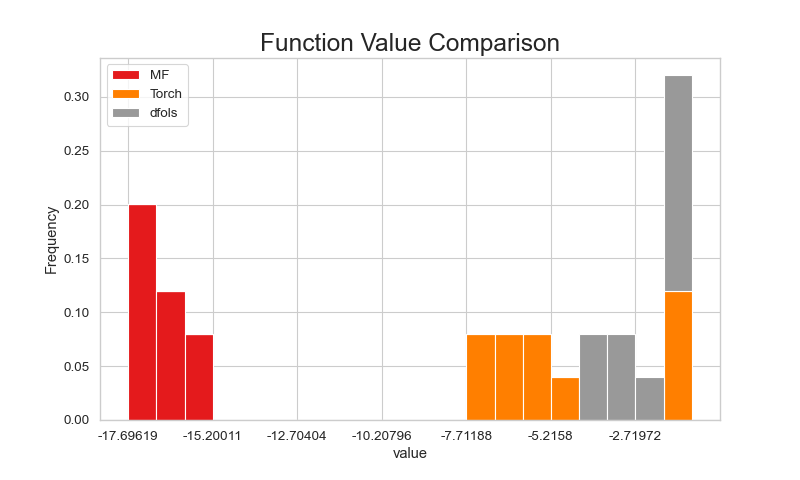
\includegraphics[width=0.5\linewidth]{valuecompare2.png}
   }
   \caption{(Best viewed in color) Comparison result of three model. Function value is viewed in log scale of difference with oracle obtained by grid search. MF achieves best precision in relatively short time. }
   \label{fig:compare2}
  \end{figure}





 \section{Benchmark Problem Set}
 \label{ap3}
 In this appendix, we provide details about benchmark from \cite{benchmark}. Rigorous formulation are as follows. 
 \begin{enumerate}
 
 \item Generalization of MAXQ
 \begin{flalign}
 \hspace{3mm}&
 \begin{array}{l}
f(\mathbf{x})=\max _{1 \leq i \leq n} x_{i}^{2} \\
x_{i}^{(1)}=i, \quad \text { for } i=1, \ldots, n / 2 \text { and } \\
x_{i}^{(1)}=-i, \quad \text { for } i=n / 2+1, \ldots, n .
\end{array}
&
\nonumber
\end{flalign}

 \item Generalization of MXHILB
 \begin{flalign}
 \hspace{3mm}&
\begin{array}{l}
f(\mathbf{x})=\max _{1 \leq i \leq n}\left|\sum_{j=1}^{n} \frac{x_{j}}{i+j-1}\right| \\
x_{i}^{(1)}=1, \quad \text { for all } i=1, \ldots, n
\end{array}
&
\nonumber
\end{flalign}

 \item Chained LQ
 \begin{flalign}
 \hspace{3mm}&
\begin{array}{l}
f(\mathbf{x})=\sum_{i=1}^{n-1} \max \left\{-x_{i}-x_{i+1},-x_{i}-x_{i+1}+\left(x_{i}^{2}+x_{i+1}^{2}-1\right)\right\} \\
x_{i}^{(1)}=-0.5, \text { for all } i=1, \ldots, n
\end{array}
&
\nonumber
\end{flalign}

 \item Chained CB3 1
 \begin{flalign}
 \hspace{3mm}&
\begin{array}{l}
f(\mathbf{x})=\sum_{i=1}^{n-1} \max \left\{x_{i}^{4}+x_{i+1}^{2},\left(2-x_{i}\right)^{2}+\left(2-x_{i+1}\right)^{2}, 2 e^{-x_{i}+x_{i+1}}\right\} \\
x_{i}^{(1)}=2, \quad \text { for all } i=1, \ldots, n
\end{array}
&
\nonumber
\end{flalign}

 \item Chained CB3 2
 \begin{flalign}
 \hspace{3mm}&
\begin{array}{l}
f(\mathbf{x})=\max \left\{\sum_{i=1}^{n-1}\left(x_{i}^{4}+x_{i+1}^{2}\right), \sum_{i=1}^{n-1}\left(\left(2-x_{i}\right)^{2}+\left(2-x_{i+1}\right)^{2}\right)\right. \\
\left.\sum_{i=1}^{n-1}\left(2 e^{-x_{i}+x_{i+1}}\right)\right\} \\
x_{i}^{(1)}=2, \quad \text { for all } i=1, \ldots, n
\end{array}
&
\nonumber
\end{flalign}

 \item Number of Active Faces
 \begin{flalign}
 \hspace{3mm}&
\begin{array}{l}
f(\mathbf{x})=\max _{1 \leq i \leq n}\left\{g\left(-\sum_{i=1}^{n} x_{i}\right), g\left(x_{i}\right)\right\} \\
\text { where } g(y)=\ln (|y|+1) \\
x_{i}^{(1)}=1, \quad \text { for all } i=1, \ldots, n
\end{array}
&
\nonumber
\end{flalign}

 \item Chained Mifflin
 \begin{flalign}
 \hspace{3mm}&
\begin{array}{l}
f(\mathbf{x})=\sum_{i=1}^{n-1}\left(-x_{i}+2\left(x_{i}^{2}+x_{i+1}^{2}-1\right)+1.75\left|x_{i}^{2}+x_{i+1}^{2}-1\right|\right) \\
x_{i}^{(1)}=-1, \quad \text { for all } i=1, \ldots, n
\end{array}
&
\nonumber
\end{flalign}

 \item Chained Crescent 1
 \begin{flalign}
 \hspace{3mm}&
\begin{aligned}
&\begin{array}{r}
f(\mathbf{x})=\max \left\{\sum_{i=1}^{n-1}\left(x_{i}^{2}+\left(x_{i+1}-1\right)^{2}+x_{i+1}-1\right)\right. \\
\left.\sum_{i=1}^{n-1}\left(-x_{i}^{2}-\left(x_{i+1}-1\right)^{2}+x_{i+1}+1\right)\right\}
\end{array}\\
&x_{i}^{(1)}=-1.5, \text { when } \bmod (i, 2)=1,(i=1, \ldots, n) \text { and }\\
&x_{i}^{(1)}=2.0, \quad \text { when } \quad \bmod (i, 2)=0,(i=1, \ldots, n) .
\end{aligned}
&
\nonumber
\end{flalign}

 \item Chained Crescent 2
 \begin{flalign}
 \hspace{3mm}&
\begin{aligned}
&\begin{aligned}
f(\mathbf{x})=\sum_{i=1}^{n-1} & \max \left\{x_{i}^{2}+\left(x_{i+1}-1\right)^{2}+x_{i+1}-1,
-x_{i}^{2}-\left(x_{i+1}-1\right)^{2}+x_{i+1}+1\right\} &
\end{aligned}\\
&x_{i}^{(1)}=-1.5, \text { when } \bmod (i, 2)=1,(i=1, \ldots, n) \text { and }\\
&x_{i}^{(1)}=2.0, \quad \text { when } \quad \bmod (i, 2)=0,(i=1, \ldots, n) .
\end{aligned}
&
\nonumber
\end{flalign}


 \end{enumerate}
 
 
 Note that problem 6 is in fact not proper here since it doesn't satisfy fully linearity \ref{secondlip}, but we keep it for completeness of the test set. For properties of the test functions, we refer to Table \ref{tab:test}.
 
 
 % Please add the following required packages to your document preamble:
% \usepackage{multirow}
\begin{table}[]
\centering
\caption{Details of test problem set. }
\label{tab:test}
\begin{tabular}{cccccc}
\hline
Index                  & Optimal Value         & Convexity      & Non-smoothness(h)                                   & $L_h$                                       & m          \\ \hline
\multicolumn{1}{c|}{1} & 0                     & Y              & \multicolumn{1}{c|}{$max(\cdot)$}                   & \multicolumn{1}{c|}{\multirow{9}{*}{1}}     & n          \\ \cline{1-4} \cline{6-6} 
\multicolumn{1}{c|}{2} & 0                     & Y              & \multicolumn{1}{c|}{$max(\left |\cdot\right|)$}     & \multicolumn{1}{c|}{}                       & n          \\ \cline{1-4} \cline{6-6} 
\multicolumn{1}{c|}{3} & $-(n-1)\sqrt{2}$      & Y              & \multicolumn{1}{c|}{$\sum max(\cdot)$}              & \multicolumn{1}{c|}{}                       & 2(n-1)     \\ \cline{1-4} \cline{6-6} 
\multicolumn{1}{c|}{4} & 2(n-1)                & Y              & \multicolumn{1}{c|}{$\sum max(\cdot)$}              & \multicolumn{1}{c|}{}                       & 3(n-1)     \\ \cline{1-4} \cline{6-6} 
\multicolumn{1}{c|}{5} & 2(n-1)                & Y              & \multicolumn{1}{c|}{$max(\cdot)$}                   & \multicolumn{1}{c|}{}                       & 3          \\ \cline{1-4} \cline{6-6} 
\multicolumn{1}{c|}{6} & 0                     & N              & \multicolumn{1}{c|}{$max(\cdot)$}                   & \multicolumn{1}{c|}{}                       & n+1        \\ \cline{1-4} \cline{6-6} 
\multicolumn{1}{c|}{7} & Varies*               & N              & \multicolumn{1}{c|}{$\left|\cdot\right|$}           & \multicolumn{1}{c|}{}                       & n-1        \\ \cline{1-4} \cline{6-6} 
\multicolumn{1}{c|}{8} & 0                     & N              & \multicolumn{1}{c|}{$max(\cdot)$}                   & \multicolumn{1}{c|}{}                       & 2          \\ \cline{1-4} \cline{6-6} 
\multicolumn{1}{c|}{9} & 0                     & N              & \multicolumn{1}{c|}{$\sum max(\cdot)$}              & \multicolumn{1}{c|}{}                       & 2(n-1)     \\ \hline
                       & \multicolumn{5}{c}{\begin{tabular}[c]{@{}c@{}}* Optimal value is approximately -6.51 for n=10, \\ -70.15 for n=100 and -706.55 for n=1000\end{tabular}} \\ \hline
\end{tabular}
\end{table}
 
 

 
 
\end{document}
